\section{Conflict Graphs and Mazurkiewicz Traces}\seclabel{ConflictGraphs}
Consider a set $\Cmd$ of commands and a binary reflexive relation $\conflict$
over $\Cmd$. We say two commands $x, y \in \Cmd$ \defword{conflict} if $(x, y)
\in \conflict$, and we say they are \defword{independent} otherwise. A
\defword{conflict graph}~\cite{mazurkiewicz1995introduction} (with respect to
$\Cmd$ and $\conflict$) is a directed acyclic graph $C = (V, E, \varphi)$ where
\begin{itemize}
  \item
    $V$ is a set of vertices;
  \item
    $E \subseteq V \times V$ is a set of edges;
  \item
    $\varphi: V \to \Cmd$ is a function that labels every vertex with a command;
    and
  \item
    for every pair of vertices $v_1, v_2 \in V$, there exists an edge between
    $v_1$ and $v_2$ if and only if $\varphi(v_1)$ and $\varphi(v_2)$ conflict.
\end{itemize}

We say $C' = (V', E', \varphi|_{V'})$ is a \defword{suffix} of $C$ if $C'$ is a
subgraph of $C$ such that for every edge $(v_1, v_2) \in E$, if $v_1 \in V'$,
then $(v_1, v_2) \in E'$.
%
An example conflict graph is shown in \figref{ExampleConflictGraph} with $\Cmd
= \set{x, y, z}$ and $\conflict = \set{(x, x), (x, y), (y, x), (x, z), (z,
x)}$. A suffix of this conflict graph is shown in \figref{ExampleSuffix}.

\begin{floatingfigure}{0.27\textwidth}
  \centering
  \tikzstyle{vertex}=[]
  \tikzstyle{arrow}=[thick, -latex]
  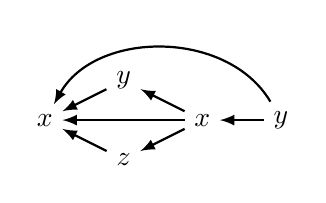
\begin{tikzpicture}
    \node[vertex] (x1) at (0, 0) {$x$};
    \node[vertex] (y1) at (1, 0.5) {$y$};
    \node[vertex] (y2) at (1, -0.5) {$z$};
    \node[vertex] (x2) at (2, 0) {$x$};
    \node[vertex] (z) at (3, 0) {$y$};

    \draw[arrow] (y1) to (x1);
    \draw[arrow] (y2) to (x1);
    \draw[arrow] (x2) to (y1);
    \draw[arrow] (x2) to (y2);
    \draw[arrow] (x2) to (x1);
    \draw[arrow, bend right=60] (z) to (x1);
    \draw[arrow] (z) to (x2);
  \end{tikzpicture}
  \caption{A conflict graph.}\figlabel{ExampleConflictGraph}
\end{floatingfigure}


We associate every conflict graph with the set of command strings that can be
obtained by a reverse topological sort of the conflict graph. For example, the
conflict graph in \figref{ExampleConflictGraph} can be reverse topological
sorted in two ways, yielding the two command strings $xyzxy$ and $xzyxy$.
Notice that these two command strings can be obtained from one another by
interchanging their second and third commands, two commands that do not
conflict. This is true in general. Any two command strings associated with a
conflict graph can be obtained from the other by repeatedly interchanging
adjacent independent commands. These sets of command strings are known as
Mazurkiewicz traces~\cite{mazurkiewicz1985semantics,
mazurkiewicz1995introduction} and formalize the orders in which replicated
state machines can execute commands while remaining in sync.

